%%%%%%%%%%%%%%%%%%%%%%%%%%%%%%%%%%%%%%%%%%%%%%%%%%%%%%%%%%%%%%%%%%%%%%%%%%%%%%%%
%
% Template license:
% CC BY-NC-SA 3.0 (http://creativecommons.org/licenses/by-nc-sa/3.0/)
%
% Adaptación para PPS UTN- FRRO por Marcelo Castello
%%%%%%%%%%%%%%%%%%%%%%%%%%%%%%%%%%%%%%%%%%%%%%%%%%%%%%%%%%%%%%%%%%%%%%%%%%%%%%%%

%----------------------------------------------------------------------------------------
%	PACKAGES AND OTHER DOCUMENT CONFIGURATIONS
%----------------------------------------------------------------------------------------

\documentclass[
11pt, % The default document font size, options: 10pt, 11pt, 12pt
%oneside, % Two side (alternating margins) for binding by default, uncomment to switch to one side
%chapterinoneline,% Have the chapter title next to the number in one single line
spanish,
singlespacing, % Single line spacing, alternatives: onehalfspacing or doublespacing
%draft, % Uncomment to enable draft mode (no pictures, no links, overfull hboxes indicated)
%nolistspacing, % If the document is onehalfspacing or doublespacing, uncomment this to set spacing in lists to single
%liststotoc, % Uncomment to add the list of figures/tables/etc to the table of contents
%toctotoc, % Uncomment to add the main table of contents to the table of contents
parskip, % Uncomment to add space between paragraphs
codirector, % Uncomment to add a codirector to the title page
headsepline, % Uncomment to get a line under the header
]{MastersDoctoralThesis} % The class file specifying the document structure


%----------------------------------------------------------------------------------------
%	INFORMACIÓN DE LA PPS
%----------------------------------------------------------------------------------------

\thesistitle{Migración de servidor de persistencia y visualización del centro de monitoreo del OES en la ciudad de Armstrong} % El título de la memoria, se usa en la carátula y se puede usar el cualquier lugar del documento con el comando \ttitle

% Nombre de la carrera, se usa en la carátula y se puede usar el cualquier lugar del documento con el comando \degreename
\posgrado{Carrera de Ingeniería Eléctrica} 


\author{Juan Perez} % Tu nombre, se usa en la carátula y se puede usar el cualquier lugar del documento con el comando \authorname

\tutor{Esp. Ing. Marcelo Castello (UTN - FRRO)} % El nombre del tutor, se usa en la carátula y se puede usar el cualquier lugar del documento con el comando \tutorname

\codirector{Nombre del supervisor de campo (pertenencia)} % El nombre del supervisor de campo si lo hubiera, se usa en la carátula y se puede usar el cualquier lugar del documento con el comando \codirname.  Para activar este campo se debe descomentar la opción "codirector" en el comando \documentclass, línea 23.

\empresa{Nombre de la empresa/institución}

\juradoUNO{Dr. Ing. } % Nombre y pertenencia del un jurado se usa en la carátula y se puede usar el cualquier lugar del documento con el comando \jur1name
\juradoDOS{Mg. Ing. } % Nombre y pertenencia del un jurado se usa en la carátula y se puede usar el cualquier lugar del documento con el comando \jur2name
%\juradoTRES{Esp. Ing. Lic. Pablo José Carlos Alonso Castillo (FCEyN UBA, FIUBA))} % Nombre y pertenencia del un jurado se usa en la carátula y se puede usar el cualquier lugar del documento con el comando \jur3name

\ciudad{ciudad de Rosario}

\fechaINICIO{agosto de 2020}
\fechaFINAL{agosto de 2021}


\keywords{Sistemas embebidos, energías renovables} % Keywords for your thesis, print it elsewhere with \keywordnames


\begin{document}


\frontmatter % Use roman page numbering style (i, ii, iii, iv...) for the pre-content pages

\pagestyle{plain} % Default to the plain heading style until the thesis style is called for the body content


%----------------------------------------------------------------------------------------
%	RESUMEN - ABSTRACT 
%----------------------------------------------------------------------------------------

\begin{abstract}
\addchaptertocentry{\abstractname} % Add the abstract to the table of contents
%
%The Thesis Abstract is written here (and usually kept to just this page). The page is kept centered vertically so can expand into the blank space above the title too\ldots
\centering

En este trabajo se describe el diseño e implementación de un sistema de ..........................El mismo surge de la necesidad de la .............

En el trabajo se aplicaron conocimientos referidos a ciberseguridad en aplicaciones, infraestructura y protocolos de comunicación para dispositivos sensores, procesamiento de mensajes, visualización y graficación de datos. 

\end{abstract}

%----------------------------------------------------------------------------------------
%	CONTENIDO DE LA PPS  - AGRADECIMIENTOS
%----------------------------------------------------------------------------------------

\begin{acknowledgements}
%\addchaptertocentry{\acknowledgementname} % Descomentando esta línea se puede agregar los agradecimientos al índice
\vspace{1.5cm}

Espacio para agradecimientos  

\end{acknowledgements}

%----------------------------------------------------------------------------------------
%	LISTA DE CONTENIDOS/FIGURAS/TABLAS
%----------------------------------------------------------------------------------------

\tableofcontents % Prints the main table of contents

\listoffigures % Prints the list of figures

\listoftables % Prints the list of tables


%----------------------------------------------------------------------------------------
%	CONTENIDO DE LA PPS  - DEDICATORIA
%----------------------------------------------------------------------------------------

%\dedicatory{\textbf{Dedicado a... [OPCIONAL]}}  % escribir acá si se desea una dedicatoria

%----------------------------------------------------------------------------------------
%	CONTENIDO DE LA PPS - CAPÍTULOS
%----------------------------------------------------------------------------------------

\mainmatter % Begin numeric (1,2,3...) page numbering

\pagestyle{thesis} % Return the page headers back to the "thesis" style

% Incluir los capítulos como archivos separados desde la carpeta Chapters

% Chapter 1

\chapter{Introducción general} % Main chapter title

\label{Chapter1} % For referencing the chapter elsewhere, use \ref{Chapter1} 
\label{IntroGeneral}

%----------------------------------------------------------------------------------------

% Define some commands to keep the formatting separated from the content 
\newcommand{\keyword}[1]{\textbf{#1}}
\newcommand{\tabhead}[1]{\textbf{#1}}
\newcommand{\code}[1]{\texttt{#1}}
\newcommand{\file}[1]{\texttt{\bfseries#1}}
\newcommand{\option}[1]{\texttt{\itshape#1}}
\newcommand{\grados}{$^{\circ}$}

%----------------------------------------------------------------------------------------

%\section{Introducción}
En este capítulo se presenta una breve introducción técnica y se describen la motivación, los objetivos, el alcance y requerimientos del trabajo.
%----------------------------------------------------------------------------------------
\section{Internet de las Cosas}
El término Internet de las Cosas (IoT) describe a una red de interconexión de objetos que incorporan software, hardware y otras tecnologías con el fin de interactuar con otros dispositivos o sistemas a través de Internet. Los objetos físicos que se conectan a esta red, van desde simples sensores de temperaturas domésticos hasta redes de sensores industriales utilizados para el mantenimiento predictivo.

De esta manera, es posible capturar información clave para la detección de patrones de comportamiento que servirán para mejorar la eficiencia de los dispositivos o sistemas a los cuales están conectados. Dada la gran cantidad de sensores y datos recopilados y la alta precisión necesaria para su tratamiento, IoT necesita de tecnologías orientadas al almacenamiento, manipulación y análisis de grandes volúmenes de datos. Una de estas tecnologías que ha penetrado a ritmo acelerado en IoT es la Inteligencia Artificial, ya que al aplicar algoritmos inteligentes, permite inferir conocimiento acerca de los sensores conectados a la red.

Esta información se hace relevante al usuario de alguna forma, ya sea por la realización de alguna acción automática como una notificación o a través de gráficos y valores actuales en los llamados \textit{dashboards} o paneles de control que muestran los datos ya procesados.

Actualmente, IoT está compuesta por una colección dispersa de redes diferentes y con distintos fines \citep{cisco}. Los automóviles, las industrias, los edificios comerciales y residenciales, tienen múltiples redes para vigilar y controlar el funcionamiento de sus sistemas. A medida que IoT evolucione, estas redes se interconectarán con la incorporación de capacidades de seguridad, análisis y administración que se podrán convertir en información y conocimiento. La figura \ref{fig:iotcisco} muestra una proyección de este concepto.

Esto abre una ventana de oportunidades para crear aplicaciones en las áreas de la automatización, el uso de sensores y la comunicación entre máquinas. 
\vspace{1cm}
\begin{figure}[htbp]
	\centering
	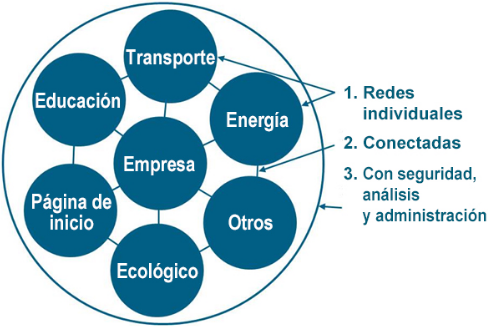
\includegraphics[width=.7\textwidth]{./Figures/iotcisco.png}
	\caption{Futuro de las redes en IoT\protect\footnotemark.}
	\label{fig:iotcisco}
\end{figure}
\vspace{1cm}
\footnotetext{Imagen tomada de: \url{https://www.cisco.com/c/dam/global/es_mx/solutions/executive/assets/pdf/internet-of-things-iot-ibsg.pdf}}

\section{Estado del arte}
Si bien en el mercado existen soluciones para vigilancia de temperaturas aplicadas al área de salud, la mayoría de estos sistemas son de origen importado. Esto hace que los costos y los servicios de mantenimiento sean elevados. Además, en general se comercializan por módulos, por lo que no se proveen soluciones completas.

Ejemplo de algunas empresas que comercializan estos sistemas en nuestro país: 
\begin{itemize}
\item Testo (Alemania) \citep{testo}. 
\item Novus (Brasil) \citep{novus}. 
\item Honeywell (USA) \citep{honeywell}.  
\item Absolut Mobile, empresa nacional que provee soluciones de telemetría a partir de módulos hardware/software importados \citep{absolutmobile}.
\item Bemakoha, empresa nacional que provee productos importados con algunos desarrollos nacionales \citep{bemakoha}.
\end{itemize}

También hay productos de origen nacional, Celsius Patagon \citep{celsius}, empresa rosarina que produce soluciones para IoT, posee un desarrollo para supervisión remota de temperatura. 
 

Casi todas las soluciones necesitan que el cliente tenga un abono mensual para el monitoreo continuo, además de adquirir el hardware correspondiente. Desde este punto de vista, el presente trabajo se destaca especialmente por incorporar una solución integral, de bajo costo, sin gastos de abono y con la característica distintiva que los datos pueden estar guardados en los servidores de la municipalidad de Rosario. Esto lo diferencia de otros sistemas similares en que los datos quedan en poder del fabricante, quien eventualmente, ofrece un portal para poder hacer una visualización. Además, al no ofrecer una solución integral, cada módulo extra incorporado representa un gasto o abono adicional.

En la tabla \ref{tab:comparacionsistemas} se muestra una comparación de algunos ítems importantes entre este trabajo y los sistemas similares de fabricación nacional o importados. En ella se ponen de manifiesto las características de bajo costo y alta prestación del sistema desarrollado.


\begin{table}[h]
	\centering
	\caption[Comparación del trabajo con productos similares importados y nacionales.]{Comparación del trabajo con productos similares importados y nacionales.}
	\begin{tabular}{l l l l}    
	\toprule
	\textbf{Beneficios}    & \textbf{Este trabajo} & \textbf{Importados}& \textbf{Nacionales}\\
	\midrule
Bajo costo del producto & Sí&No &Sí\\
Solución integral& Sí&No &No\\	
No requiere abono mensual & Sí&No &No\\	
No requiere hardware adicional& Sí&No &No\\	
Datos en servidores propios& Sí&No &No\\	
		\bottomrule
		\hline
	\end{tabular}
	\label{tab:comparacionsistemas}
\end{table}

\section{Motivación}
\label{}
El presente proyecto está dirigido a solucionar una problemática existente en la municipalidad de Rosario, donde en el área salud pública funcionan  hospitales, centros de salud, droguerías y bancos de sangre. Todos estos efectores necesitan, para almacenar los insumos médicos, sistemas de refrigeración que provean alta confiabilidad en su prestación.
El buen funcionamiento de estos sistemas es afectado a menudo por cortes de energía, mermas en el rendimiento del equipo compresor, o pérdidas en el sello, ya sea por desgaste de burletes o puertas mal cerradas.
En el área de salud esto resulta crítico puesto que productos medicinales, como hemoproductos o vacunas, pueden perder la eficacia médica. Esto no sólo se traduce en pérdidas económicas, sino también implica que los tratamientos sobre las personas pueden no ser efectivos o que no puedan ser accedidos por la pérdida del material, con el consecuente impacto social que esto representa para el municipio. 
Además, la Administración Nacional de Medicamentos Alimentos y Tecnología Médica (ANMAT), a través de la disposición: ``Buenas Prácticas de Distribución de Medicamentos'', resolución Nº 2069/2018 \citep{anmat}, define un conjunto de prácticas para el transporte y almacenamiento de productos farmacéuticos donde exige trazabilidad, equipamiento para el control y registro continuo de temperaturas con el fin de asegurar las condiciones ambientales de almacenamiento de tales productos. 

La medición a distancia, continua y en tiempo real de estas temperaturas, sumado a un sistema de alerta, aseguran las condiciones legales, minimizan los riesgos y garantizan la disponibilidad de hemoproductos y vacunas seguros en el momento y lugar en que se requieran.

Los equipos y software disponibles en plaza, en su mayoría, son de origen extranjero y su utilización -además de onerosa- implica una dependencia con los fabricantes en términos económicos pero también de criterios. En otras palabras, para trabajar con estos recursos se deben seguir criterios técnico-económicos diseñados para otras latitudes y otras condiciones. Se deben realizar adaptaciones y aproximaciones que implican tareas adicionales y que no siempre son del todo efectivas. El personal destinado a estas tareas debe entrenarse, lo que implica tiempo y esfuerzo. Este entrenamiento debe reforzarse cada vez que el propietario del sistema decide algún cambio o actualización. Por consiguiente, es menester redirigir este esfuerzo a tareas más provechosas.
Se requiere para ello, el desarrollo de tecnología propia destinada a este fin, que pueda ser adaptada a las necesidades de los investigadores locales para evitar la dependencia tecnológica en equipos y en software y reducir en todo lo posible las erogaciones durante la investigación.

\section{Objetivos y alcance}
\label{objetivos}
El propósito de este trabajo es poner en marcha un sistema de registro y visualización de temperaturas para refrigeradores críticos del área salud, con el objetivo de minimizar los riesgos de pérdida de material, mantener la calidad y eficacia médica de los productos y asegurar las condiciones legales exigidas por la autoridad competente.

La solución se compone de las siguientes partes:
\begin{itemize}
\item medición de la temperatura.
\item transporte de los datos.
\item lógica de procesamiento y persistencia de datos.
\item visualización y alarmas.
\end{itemize}


En el trabajo se diseñaron los componentes fundamentales para que el sistema sea capaz de realizar una vigilancia de temperatura de heladeras y freezers pertenecientes a distintos efectores de salud de la ciudad de Rosario. 

Para ello se desarrollaron las siguientes actividades:

\begin{itemize}
\item producción de las placas de circuito impreso para los nodos sensores de temperatura.
\item instalación y configuración de un servidor para proveer la visualización de los datos capturados por los sensores.
\item creación de reglas lógicas para originar las alarmas.
\item instalación de una base de datos en el servidor donde se almacenan las temperaturas y las configuraciones del sistema.
\item configuración de paneles de visualización de temperatura y estado para cada dispositivo conectado al sistema.
\item configuración del envío de las notificaciones de alarmas.
\end{itemize}

Quedan fuera del alcance del trabajo las siguientes características:
\begin{itemize}
\item la provisión de la infraestructura para el transporte de los datos: puntos de acceso a Internet y conexiones a Internet para cada área donde estarán emplazados los sensores.
\item las certificaciones emitidas por las autoridades competentes.
\item el desarrollo de sensores aptos para su instalación en equipos ultrafreezer (-70°C).
\item el almacenamiento de los valores de temperaturas en memorias externas.
\item el uso de baterías para su funcionamiento.
\end{itemize}



\section{Requerimientos}
\label{alcance}


Las actividades mencionadas en la sección \ref{alcance} fueron diagramadas en base a los requerimientos planteados en la planificación. Los mismos se listan a continuación.

\begin{enumerate}
\item Requerimientos de hardware de los nodos
	\begin{enumerate}
	\item Cada nodo estará compuesto por un microcontrolador, un elemento sensor de temperatura y la electrónica asociada para su funcionamiento.
	\item El microcontrolador utilizado deberá estar en fase de producción activa.
	\item El microcontrolador deberá contener capa física WiFi.	
	\item El elemento sensor deberá tener un rango de medición entre -50 y 100 ºC.
	\item El nodo deberá incluir en su circuito un filtro activo de 2º orden para filtrar las componentes de alta frecuencia de la entrada de temperatura.
	\item El nodo deberá incorporar indicadores luminosos de conexión con la red WiFi, conexión con el servidor central e indicador de fuera de rango de temperatura.	
	\end{enumerate}
	
\item Requerimientos del software de los nodos
	\begin{enumerate}
	\item Deberá contener un conjunto de parámetros que identifiquen de forma unívoca al sensor dentro del sistema.	
	\item Los parámetros se deberán almacenar en memoria no volátil.
	\item Deberá gestionar el procesamiento de los valores de temperatura: muestreo cada segundo y promediado cada 600 segundos.	
	\item Deberá incluir parámetros de calibración como offset y ganancia para su futuro contraste con un instrumento patrón.
	\item El nodo deberá incorporar una página web para configuración de parámetros específicos/calibración del sensor.
	\item Deberá incorporar un sistema de actualización remota del firmware.
    \item Deberá ser capaz de conectar distintos modelos de sensores de temperatura.
	\end{enumerate}	
	
\item Requerimientos de seguridad informática
	\begin{enumerate}
	\item La transmisión de los datos se deberá realizar con encriptación, utilizando para ello protocolos de seguridad.
	\item El acceso al sistema de visualización deberá ser con usuario y contraseña.
	\item El acceso a la página web del sensor deberá ser con usuario y contraseña.
	\end{enumerate}	

\item Requerimientos del cliente
	\begin{enumerate}
	\item El sistema de visualización debe incluir roles para distintos usuarios.
		\begin{enumerate}
		\item Rol Administrador: podrá dar alta a usuarios y cambiar sus roles.
	     \item Rol Jefe: podrá cambiar parámetros, visualizar series de tiempo y recibir alertas.
	     \item Rol Operador: sólo podrá visualizar series de tiempo y recibir alertas.
	     \end{enumerate}
	\item El sistema deberá prever la incorporación de otras variables a monitorear, que serán materia de desarrollos futuros de sensores.
	\item El sistema de visualización deberá mostrar claramente la estructura jerárquica geográfica de la empresa.	
	\item El sistema deberá ser escalable para implementar nuevas áreas a monitorear.
		\end{enumerate}
		
\item Requerimientos del sistema de visualización
    \begin{enumerate}
	\item Deberá mostrar la temperatura.
	\item Deberá mostrar el estado del dispositivo que puede ser \textit{online} o fuera de rango.
	\item Deberá mostrar la fecha y hora de la última telemetría enviada al servidor.
	\item Deberá mostrar la configuración de los parámetros de alertas (rangos de temperatura).
	\item Deberá mostrar una vista rápida de los sensores fuera de rango mediante plano en pantalla del área.
	\item Deberá mostrar una tabla con el histórico de alarmas por cada sensor.
    \item Deberá mostrar mediante gráficas la evolución de las temperaturas en el dominio del tiempo con entorno configurable.
    \item Deberá mostrar el lugar de emplazamiento del dispositivo.
	\end{enumerate}	
    

\item Requerimientos de las alarmas
	\begin{enumerate}
	\item Deberá enviar las alarmas discriminadas por efector/área.
	\item Deberá enviar notificaciones ante desplazamientos de la temperatura por encima del rango.
	\item Deberá enviar notificaciones ante desplazamientos de la temperatura por debajo del rango.
	\item Deberá enviar notificaciones ante desconexiones del dispositivo sensor.
	\item Deberá enviar notificaciones ante recupero de la conexión del dispositivo sensor.
	 \end{enumerate}	 

\item Requerimientos de compras
	\begin{enumerate}
	\item Se deberá utilizar la gestión de compras directas para elementos con presupuesto menor a {\$10.000}.
	\item Se deberán realizar las gestiones correspondiente para realizar compras en el exterior.
	\end{enumerate}
\end{enumerate}




%----------------------------------------------------------------------------------------





% Chapter 2

\chapter{Marco de referencia} % Main chapter title

\label{Chapter2} % For referencing the chapter elsewhere, use \ref{Chapter2} 
\label{Marco de referencia}

%----------------------------------------------------------------------------------------

% Define some commands to keep the formatting separated from the content 
\newcommand{\keyword}[1]{\textbf{#1}}
\newcommand{\tabhead}[1]{\textbf{#1}}
\newcommand{\code}[1]{\texttt{#1}}
\newcommand{\file}[1]{\texttt{\bfseries#1}}
\newcommand{\option}[1]{\texttt{\itshape#1}}
\newcommand{\grados}{$^{\circ}$}

%----------------------------------------------------------------------------------------
 
% Chapter 3

\chapter{Ejecución del plan de trabajo} % Main chapter title

\label{Chapter3} % For referencing the chapter elsewhere, use \ref{Chapter3} 
\label{Ejecución del plan de trabajo}

%----------------------------------------------------------------------------------------

% Define some commands to keep the formatting separated from the content 
\newcommand{\keyword}[1]{\textbf{#1}}
\newcommand{\tabhead}[1]{\textbf{#1}}
\newcommand{\code}[1]{\texttt{#1}}
\newcommand{\file}[1]{\texttt{\bfseries#1}}
\newcommand{\option}[1]{\texttt{\itshape#1}}
\newcommand{\grados}{$^{\circ}$}

%----------------------------------------------------------------------------------------

% Chapter 4

\chapter{Resultados y conclusiones} % Main chapter title

\label{Chapter4} % For referencing the chapter elsewhere, use \ref{Chapter4} 

%----------------------------------------------------------------------------------------

\section{Sección 1 del capítulo 4} 
% Chapter 4

\chapter{Vinculación del proyecto con las materias de la carrera} % Main chapter title
\label{Chapter5} % For referencing the chapter elsewhere, use \ref{Chapter4} 

Este aspecto resulta muy importante y permite al alumno y al lector del informe relacionar y conocer qué tipo de conocimiento teórico y práctico impartido durante su especialidad, fue necesario para desarrollar una determinada actividad. En principio, la idea es asociar cada uno de los objetivos específicos de la Practica Profesional a una cátedra o a un conjunto de cátedras, para lo que se sugiere que el alumno recurra a una tabla o matriz resumen. Adicionalmente, el alumno podrá incluir detalles sobre aspectos teórico-prácticos estudiados en dichas cátedras que en algún momento fueron requeridos para el desarrollo del plan de trabajo; esto exigirá la inclusión de las referencias que hayan sido consultadas.

\section{Sección 1 del capítulo 5} 
% Chapter 4

\chapter{Lecciones aprendidas y recomendaciones} % Main chapter title

\label{Chapter6} % For referencing the chapter elsewhere, use \ref{Chapter4} 


%----------------------------------------------------------------------------------------

\section{Sección 1 del capítulo 6}

%----------------------------------------------------------------------------------------
%	CONTENIDO DE LA PPS  - APÉNDICES
%----------------------------------------------------------------------------------------

\appendix % indicativo para indicarle a LaTeX los siguientes "capítulos" son apéndices

% Incluir los apéndices de la memoria como archivos separadas desde la carpeta Appendices
% Descomentar las líneas a medida que se escriben los apéndices


% Appendix A

\chapter{Título de apéndice} % Main appendix title

\label{AppendixA} % For referencing this appendix elsewhere, use \ref{AppendixA}

Contenido del apéndice A

%
% Appendix B

\chapter{Guía detallada de LaTex} % Main appendix title

\label{AppendixB} % For referencing this appendix elsewhere, use \ref{AppendixA}


%----------------------------------------------------------------------------------------
\section{Aprendiendo \LaTeX{}}

\LaTeX{} no es \textsc{WYSIWYG} (What You See is What You Get), a diferencia de los procesadores de texto como Microsoft Word o Pages de Apple o incluso LibreOffice en el mundo open-source. En lugar de ello, un documento escrito para \LaTeX{} es en realidad un archivo de texto simple o llano que \emph{no contiene formato} . Nosotros le decimos a \LaTeX{} cómo deseamos que se aplique el formato en el documento final escribiendo comandos simples entre el texto, por ejemplo, si quiero usar texto en itálicas para dar énfasis, escribo \verb|\it{texto}| y pongo el texto que quiero en itálicas entre medio de las llaves. Esto significa que \LaTeX{} es un lenguaje del tipo \enquote{mark-up}, muy parecido a HTML.

\subsection{Una introducción (no tan corta) a \LaTeX{}}

Si sos nuevo en \LaTeX{}, hay un muy buen libro electrónico - disponible gratuitamente en Internet como un archivo PDF - llamado, \enquote{A (not so short) Introduction to \LaTeX{}}. El título del libro es generalmente acortado a simplemente \emph{lshort}. Puede descargar la versión más reciente en inglés (ya que se actualiza de vez en cuando) desde aquí:
\url{http://www.ctan.org/tex-archive/info/lshort/english/lshort.pdf}

Se puede encontrar la versión en español en la lista en esta página: \url{http://www.ctan.org/tex-archive/info/lshort/}

\subsubsection{Una subsubsección}

Acá tiene un ejemplo de una ``subsubsección'' que es el cuarto nivel de ordenamiento del texto, después de capítulo, sección y subsección.  Como se puede ver, las subsubsecciones no van numeradas en el cuerpo del documento ni en el índice.  El formato está definido por la plantilla y no debe ser modificado.

\subsection{Guía matemática rápida para \LaTeX{}}

Si estás escribiendo un documento con mucho contenido matemático, entonces es posible que desees leer el documento de la AMS (American Mathematical Society) llamado, \enquote{A Short Math Guide for \LaTeX{}}. Se puede encontrar en línea en el siguiente link: \url{http://www.ams.org/tex/amslatex.html} en la sección \enquote{Additional Documentation} hacia la parte inferior de la página.


%----------------------------------------------------------------------------------------

\section{Utilizando esta plantilla}

Si estás familiarizado con \LaTeX{}, entonces podés explorar la estructura de directorios de esta plantilla y proceder a personalizarla agregando tu información en el bloque \emph{INFORMACIÓN DE LA PORTADA} en el archivo \file{pps.tex}.  

Se puede continuar luego modificando el resto de los archivos siguiendo los lineamientos que se describen en la sección \ref{sec:FillingFile} en la página \pageref{sec:FillingFile}.


Si sos nuevo en \LaTeX{}, se recomienda que continúes leyendo el documento ya que contiene información básica para aprovechar el potencial de esta herramienta.


%----------------------------------------------------------------------------------------

\section{Qué incluye esta plantilla}

\subsection{Carpetas}

Esta plantilla se distribuye como una único archivo .zip que se puede descomprimir en varios archivos y carpetas. Asimismo, se puede consultar el repositorio git para obtener la última versión de los archivos, \url{https://github.com/mcastellogh/Plantilla-PPS-UTN-FRRO}. Los nombres de las carpetas son, o pretender ser, auto-explicativos.

\keyword{Appendices} -- Esta es la carpeta donde se deben poner los apéndices. Cada apéndice debe ir en su propio archivo \file{.tex}. Se incluye un ejemplo y una plantilla en la carpeta.

\keyword{Chapters} -- Esta es la carpeta donde se deben poner los capítulos de la pps. Cada capítulo debe ir un su propio archivo \file{.tex} por separado.  Se ofrece por defecto, la siguiente estructura de capítulos y se recomienda su utilización dentro de lo posible:

\begin{itemize}
\item Capítulo 1: Introducción general.	
\item Capítulo 2: Marco de referencia.
\item Capítulo 3: Ejecución del plan de trabajo.
\item Capítulo 4: Resultados y Conclusiones.
\item Capítulo 5: Vinculación del proyecto con las materias de la carrera.
\item Capítulo 6: Lecciones aprendidas y recomendaciones.
\end{itemize}

Esta estructura de capítulos es la que se recomienda para las PPS de la carrera.

\keyword{Figures} -- Esta carpeta contiene todas las figuras de la PPS.  Estas son las versiones finales de las imágenes que van a ser incluidas en la PPS.  Pueden ser imágenes en formato \textit{raster}\footnote{\url{https://en.wikipedia.org/wiki/Raster_graphics}} como \file{.png}, \file{.jpg} o en formato vectoriales\footnote{\url{https://en.wikipedia.org/wiki/Vector_graphics}} como \file{.pdf}, \file{.ps}.  Se debe notar que utilizar imágenes vectoriales disminuye notablemente el peso del documento final y acelera el tiempo de compilación por lo que es recomendable su utilización siempre que sea posible.

\subsection{Archivos}

También están incluidos varios archivos, la mayoría de ellos son de texto plano y se puede ver su contenido en un editor de texto. Después de la compilación inicial, se verá que más archivos auxiliares son creados por \ LaTeX{} o BibTeX, pero son de uso interno y no es necesario hacer nada en particular con ellos.  Toda la información necesaria para compilar el documento se encuentra en los archivos \file{.tex}, \file{.bib}, \file{.cls} y en las imágenes de la carpeta Figures.

\keyword{referencias.bib} - este es un archivo importante que contiene toda la información de referencias bibliográficas que se utilizarán para las citas en la pps en conjunto con BibTeX. Usted puede escribir las entradas bibliográficas en forma manual, aunque existen también programas de gestión de referencias que facilitan la creación y gestión de las referencias y permiten exportarlas en formato BibTeX.  También hay disponibles sitios web como \url{books.google.com} que permiten obtener toda la información necesaria para una cita en formato BibTeX. Ver sección \ref{sec:biblio}

\keyword{MastersDoctoralThesis.cls} -- este es un archivo importante. Es el archivos con la clase que le informa a \LaTeX{} cómo debe dar formato a la pps. El usuario de la plantilla no debería necesitar modificar nada de este archivo.

\keyword{pps.pdf} -- esta es su pps con una tipografía bellamente compuesta (en formato de archivo PDF) creado por \LaTeX{}. Se distribuye con la plantilla y después de compilar por primera vez sin hacer ningún cambio se debería obtener una versión idéntica a este documento.

\keyword{pps.tex} -- este es un archivo importante. Este es el archivo que tiene que compilar \LaTeX{} para producir la pps como un archivo PDF. Contiene un marco de trabajo y estructuras que le indican a \LaTeX{} cómo diagramar la pps.  Está altamente comentado para que se pueda entender qué es lo que realiza cada línea de código y por qué está incluida en ese lugar.  En este archivo se debe completar la información personalizada de las primeras sección según se indica en la sección \ref{sec:FillingFile}.

Archivos que \emph{no} forman parte de la distribución de la plantilla pero que son generados por \LaTeX{} como archivos auxiliares necesarios para la producción de la pps.pdf son:

\keyword{pps.aux} -- este es un archivo auxiliar generado por \LaTeX{}, si se borra \LaTeX{} simplemente lo regenera cuando se compila el archivo principal \file{pps.tex}.

\keyword{pps.bbl} -- este es un archivo auxiliar generado por BibTeX, si se borra BibTeX simplemente lo regenera cuando se compila el archivo principal \file{pps.tex}. Mientras que el archivo \file{.bib} contiene todas las referencias que hay, este archivo \file{.bbl} contine sólo las referencias que han sido citadas y se utiliza para la construcción de la bibiografía.

\keyword{pps.blg} -- este es un archivo auxiliar generado por BibTeX, si se borra BibTeX simplemente lo regenera cuando se compila el archivo principal \file{pps.tex}.

\keyword{pps.lof} -- este es un archivo auxiliar generado por \LaTeX{}, si se borra \LaTeX{} simplemente lo regenera cuando se compila el archivo principal \file{pps.tex}.  Le indica a \LaTeX{} cómo construir la sección \emph{Lista de Figuras}.
 
\keyword{pps.log} --  este es un archivo auxiliar generado por \LaTeX{}, si se borra \LaTeX{} simplemente lo regenera cuando se compila el archivo principal \file{pps.tex}. Contiene mensajes de \LaTeX{}. Si se reciben errores o advertencias durante la compilación, se guardan en este archivo \file{.log}.

\keyword{pps.lot} -- este es un archivo auxiliar generado por \LaTeX{}, si se borra \LaTeX{} simplemente lo regenera cuando se compila el archivo principal \file{pps.tex}.  Le indica a \LaTeX{} cómo construir la sección \emph{Lista de Tablas}.

\keyword{pps.out} -- este es un archivo auxiliar generado por \LaTeX{}, si se borra \LaTeX{} simplemente lo regenera cuando se compila el archivo principal \file{pps.tex}.

De esta larga lista de archivos, sólo aquellos con la extensión \file{.bib}, \file{.cls} y \file{.tex} son importantes.  Los otros archivos auxiliares pueden ser ignorados o borrados ya que \LaTeX{} y BibTeX los regenerarán durante la compilación.

%----------------------------------------------------------------------------------------

\section{Entorno de trabajo}

Ante de comenzar a editar la plantilla debemos tener un editor \LaTeX{} instalado en nuestra computadora.  En forma análoga a lo que sucede en lenguaje C, que se puede crear y editar código con casi cualquier editor, existen ciertos entornos de trabajo que nos pueden simplificar mucho la tarea.  En este sentido, se recomienda, sobre todo para los principiantes en \LaTeX{} la utilización de TexMaker, un programa gratuito y multi-plantaforma que está disponible tanto para windows como para sistemas GNU/linux.

La versión más reciente de TexMaker es la 4.5 y se puede descargar del siguiente link: \url{http://www.xm1math.net/texmaker/download.html}. Se puede consultar el manual de usuario en el siguiente link: \url{http://www.xm1math.net/texmaker/doc.html}.
 

\subsection{Paquetes adicionales}

Si bien durante el proceso de instalación de TexMaker, o cualquier otro editor que se haya elegido, se instalarán en el sistema los paquetes básicos necesarios para trabajar con \LaTeX{}, la plantilla de los trabajos de Especialización y Maestría requieren de paquete adicionales.

Se indican a continuación los comandos que se deben introducir en la consola de Ubuntu (ctrl + alt + t) para instalarlos:

\begin{lstlisting}[language=bash]
  $ sudo apt install texlive-lang-spanish texlive-science 
  $ sudo apt install texlive-bibtex-extra biber
  $ sudo apt install texlive texlive-fonts-recommended
  $ sudo apt install texlive-latex-extra
\end{lstlisting}


\subsection{Configurando TexMaker}



Una vez instalado el programa y los paquetes adicionales se debe abrir el archivo pps.tex con el editor para ver una pantalla similar a la que se puede apreciar en la figura \ref{fig:texmaker}. 

\vspace{1cm}

\begin{figure}[htbp]
	\centering
	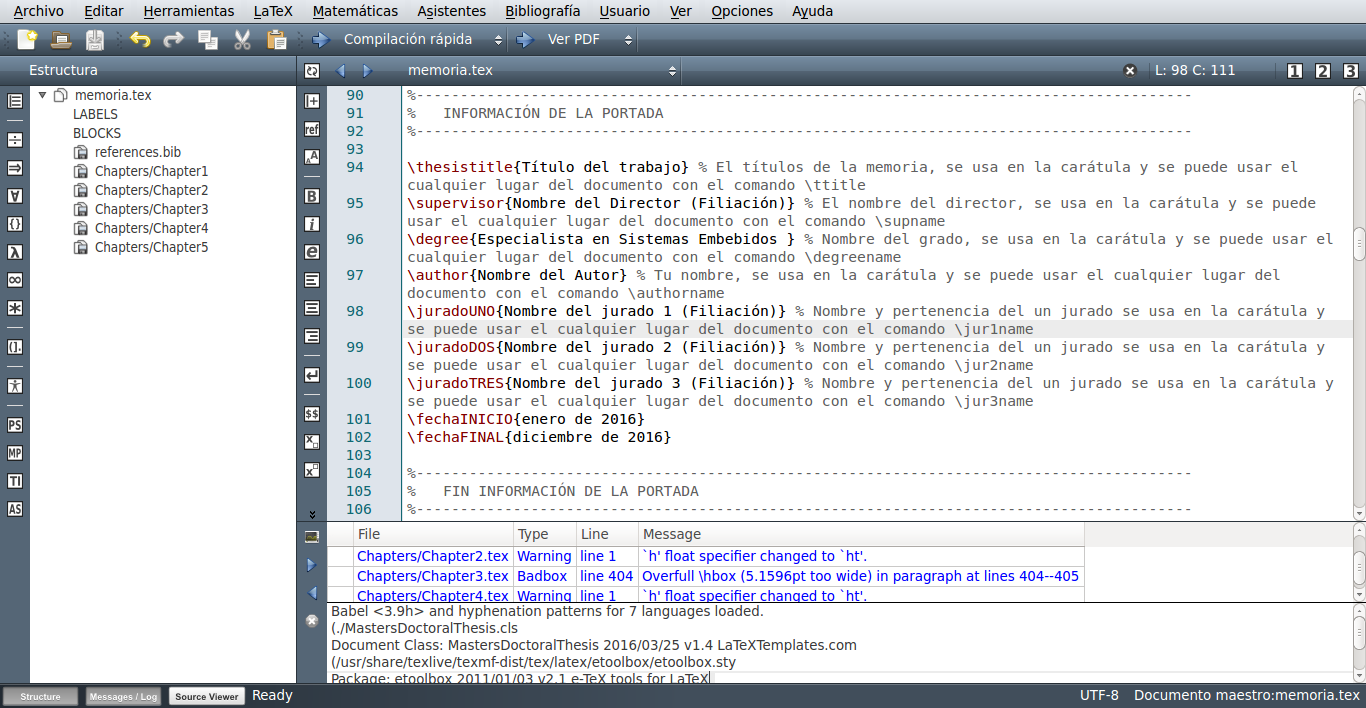
\includegraphics[width=.99\textwidth]{./Figures/texmaker.png}
	\caption{Entorno de trabajo de texMaker.}
	\label{fig:texmaker}
\end{figure}

\vspace{1cm}

Notar que existe una vista llamada Estructura a la izquierda de la interfaz que nos permite abrir desde dentro del programa los archivos individuales de los capítulos.  A la derecha se encuentra una vista con el archivo propiamente dicho para su edición. Hacia la parte inferior se encuentra una vista del log con información de los resultados de la compilación.  En esta última vista pueden aparecen advertencias o \textit{warning}, que normalmente pueden ser ignorados, y los errores que se indican en color rojo y deben resolverse para que se genere el PDF de salida.

Recordar que el archivo que se debe compilar con PDFLaTeX es \file{pps.tex}, si se tratara de compilar alguno de los capítulos saldría un error.  Para salvar la molestia de tener que cambiar de archivo para compilar cada vez que se realice una modificación en un capítulo, se puede definir el archivo \file{pps.tex} como ``documento maestro'' yendo al menú opciones -> ``definir documento actual como documento maestro'', lo que permite compilar con PDFLaTeX pps.tex directamente desde cualquier archivo que se esté modificando . Se muestra esta opción en la figura \ref{fig:docMaestro}.

\begin{figure}[h]
	\centering
	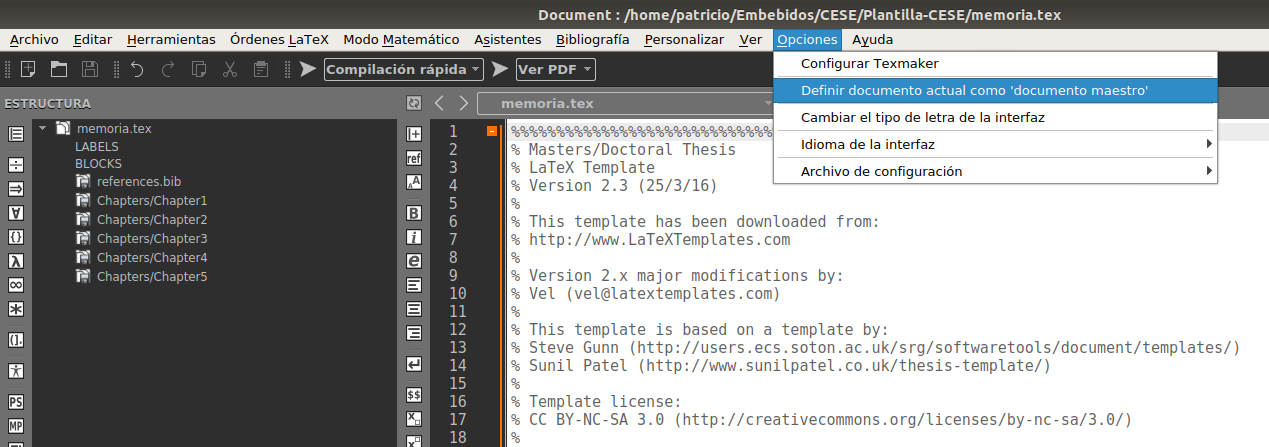
\includegraphics[width=\textwidth]{./Figures/docMaestro.png}
	\caption{Definir pps.tex como documento maestro.}
	\label{fig:docMaestro}
\end{figure}

En el menú herramientas se encuentran las opciones de compilación.  Para producir un archivo PDF a partir de un archivo .tex se debe ejecutar PDFLaTeX (el shortcut es F6). Para incorporar nueva bibliografía se debe utilizar la opción BibTeX del mismo menú herramientas (el shortcut es F11).

Notar que para actualizar las tablas de contenidos se debe ejecutar PDFLaTeX dos veces.  Esto se debe a que es necesario actualizar algunos archivos auxiliares antes de obtener el resultado final.  En forma similar, para actualizar las referencias se debe ejecutar primero PDFLaTeX, después BibTeX y finalmente PDFLaTeX dos veces por idénticos motivos.

\section{Personalizando la plantilla, el archivo \file{pps.tex}}
\label{sec:FillingFile}

Para personalizar la plantilla se debe incorporar la información propia en los distintos archivos \file{.tex}. 

Primero abrir \file{pps.tex} con TexMaker (o el editor de su preferencia). Se debe ubicar dentro del archivo el bloque de código titulado \emph{INFORMACIÓN DE LA PORTADA} donde se deben incorporar los primeros datos personales con los que se construirá automáticamente la portada.


%----------------------------------------------------------------------------------------

\section{El código del archivo \file{pps.tex} explicado}

El archivo \file{pps.tex} contiene la estructura del documento y es el archivo de mayor jerarquía de la pps.  Podría ser equiparable a la función \emph{main()} de un programa en C, o mejor dicho al archivo fuente .c donde se encuentra definida la función main().

La estructura básica de cualquier documento de \LaTeX{} comienza con la definición de clase del documento, es seguida por un preámbulo donde se pueden agregar funcionalidades con el uso de \texttt{paquetes} (equiparables a bibliotecas de C), y finalmente, termina con el cuerpo del documento, donde irá el contenido de la pps.

\lstset{%
  basicstyle=\small\ttfamily,
  language=[LaTeX]{TeX}
}

\begin{lstlisting}
\documentclass{article}  <- Definicion de clase
\usepackage{listings}	 <- Preambulo

\begin{document}	 <- Comienzo del contenido propio 
	Hello world!
\end{document}
\end{lstlisting}


El archivo \file{pps.tex} se encuentra densamente comentado para explicar qué páginas, secciones y elementos de formato está creando el código \LaTeX{} en cada línea. El código está dividido en bloques con nombres en mayúsculas para que resulte evidente qué es lo que hace esa porción de código en particular. Inicialmente puede parecer que hay mucho código \LaTeX{}, pero es principalmente código para dar formato a la pps por lo que no requiere intervención del usuario de la plantilla.  Sí se deben personalizar con su información los bloques indicados como:

\begin{itemize}
	\item Informacion de la pps
	\item Resumen
	\item Agradecimientos
	\item Dedicatoria
\end{itemize}

El índice de contenidos, las listas de figura de tablas se generan en forma automática y no requieren intervención ni edición manual por parte del usuario de la plantilla. 

En la parte final del documento se encuentran los capítulos y los apéndices.  Por defecto se incluyen los 6 capítulos propuestos que se encuentran en la carpeta /Chapters. Cada capítulo se debe escribir en un archivo .tex separado y se debe poner en la carpeta \emph{Chapters} con el nombre \file{Chapter1}, \file{Chapter2}, etc\ldots El código para incluir capítulos desde archivos externos se muestra a continuación.

\begin{verbatim}
	% Chapter 1

\chapter{Introducción general} % Main chapter title

\label{Chapter1} % For referencing the chapter elsewhere, use \ref{Chapter1} 
\label{IntroGeneral}

%----------------------------------------------------------------------------------------

% Define some commands to keep the formatting separated from the content 
\newcommand{\keyword}[1]{\textbf{#1}}
\newcommand{\tabhead}[1]{\textbf{#1}}
\newcommand{\code}[1]{\texttt{#1}}
\newcommand{\file}[1]{\texttt{\bfseries#1}}
\newcommand{\option}[1]{\texttt{\itshape#1}}
\newcommand{\grados}{$^{\circ}$}

%----------------------------------------------------------------------------------------

%\section{Introducción}
En este capítulo se presenta una breve introducción técnica y se describen la motivación, los objetivos, el alcance y requerimientos del trabajo.
%----------------------------------------------------------------------------------------
\section{Internet de las Cosas}
El término Internet de las Cosas (IoT) describe a una red de interconexión de objetos que incorporan software, hardware y otras tecnologías con el fin de interactuar con otros dispositivos o sistemas a través de Internet. Los objetos físicos que se conectan a esta red, van desde simples sensores de temperaturas domésticos hasta redes de sensores industriales utilizados para el mantenimiento predictivo.

De esta manera, es posible capturar información clave para la detección de patrones de comportamiento que servirán para mejorar la eficiencia de los dispositivos o sistemas a los cuales están conectados. Dada la gran cantidad de sensores y datos recopilados y la alta precisión necesaria para su tratamiento, IoT necesita de tecnologías orientadas al almacenamiento, manipulación y análisis de grandes volúmenes de datos. Una de estas tecnologías que ha penetrado a ritmo acelerado en IoT es la Inteligencia Artificial, ya que al aplicar algoritmos inteligentes, permite inferir conocimiento acerca de los sensores conectados a la red.

Esta información se hace relevante al usuario de alguna forma, ya sea por la realización de alguna acción automática como una notificación o a través de gráficos y valores actuales en los llamados \textit{dashboards} o paneles de control que muestran los datos ya procesados.

Actualmente, IoT está compuesta por una colección dispersa de redes diferentes y con distintos fines \citep{cisco}. Los automóviles, las industrias, los edificios comerciales y residenciales, tienen múltiples redes para vigilar y controlar el funcionamiento de sus sistemas. A medida que IoT evolucione, estas redes se interconectarán con la incorporación de capacidades de seguridad, análisis y administración que se podrán convertir en información y conocimiento. La figura \ref{fig:iotcisco} muestra una proyección de este concepto.

Esto abre una ventana de oportunidades para crear aplicaciones en las áreas de la automatización, el uso de sensores y la comunicación entre máquinas. 
\vspace{1cm}
\begin{figure}[htbp]
	\centering
	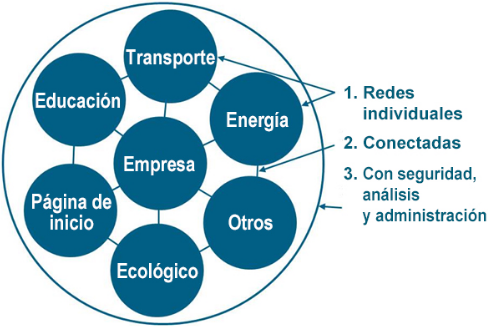
\includegraphics[width=.7\textwidth]{./Figures/iotcisco.png}
	\caption{Futuro de las redes en IoT\protect\footnotemark.}
	\label{fig:iotcisco}
\end{figure}
\vspace{1cm}
\footnotetext{Imagen tomada de: \url{https://www.cisco.com/c/dam/global/es_mx/solutions/executive/assets/pdf/internet-of-things-iot-ibsg.pdf}}

\section{Estado del arte}
Si bien en el mercado existen soluciones para vigilancia de temperaturas aplicadas al área de salud, la mayoría de estos sistemas son de origen importado. Esto hace que los costos y los servicios de mantenimiento sean elevados. Además, en general se comercializan por módulos, por lo que no se proveen soluciones completas.

Ejemplo de algunas empresas que comercializan estos sistemas en nuestro país: 
\begin{itemize}
\item Testo (Alemania) \citep{testo}. 
\item Novus (Brasil) \citep{novus}. 
\item Honeywell (USA) \citep{honeywell}.  
\item Absolut Mobile, empresa nacional que provee soluciones de telemetría a partir de módulos hardware/software importados \citep{absolutmobile}.
\item Bemakoha, empresa nacional que provee productos importados con algunos desarrollos nacionales \citep{bemakoha}.
\end{itemize}

También hay productos de origen nacional, Celsius Patagon \citep{celsius}, empresa rosarina que produce soluciones para IoT, posee un desarrollo para supervisión remota de temperatura. 
 

Casi todas las soluciones necesitan que el cliente tenga un abono mensual para el monitoreo continuo, además de adquirir el hardware correspondiente. Desde este punto de vista, el presente trabajo se destaca especialmente por incorporar una solución integral, de bajo costo, sin gastos de abono y con la característica distintiva que los datos pueden estar guardados en los servidores de la municipalidad de Rosario. Esto lo diferencia de otros sistemas similares en que los datos quedan en poder del fabricante, quien eventualmente, ofrece un portal para poder hacer una visualización. Además, al no ofrecer una solución integral, cada módulo extra incorporado representa un gasto o abono adicional.

En la tabla \ref{tab:comparacionsistemas} se muestra una comparación de algunos ítems importantes entre este trabajo y los sistemas similares de fabricación nacional o importados. En ella se ponen de manifiesto las características de bajo costo y alta prestación del sistema desarrollado.


\begin{table}[h]
	\centering
	\caption[Comparación del trabajo con productos similares importados y nacionales.]{Comparación del trabajo con productos similares importados y nacionales.}
	\begin{tabular}{l l l l}    
	\toprule
	\textbf{Beneficios}    & \textbf{Este trabajo} & \textbf{Importados}& \textbf{Nacionales}\\
	\midrule
Bajo costo del producto & Sí&No &Sí\\
Solución integral& Sí&No &No\\	
No requiere abono mensual & Sí&No &No\\	
No requiere hardware adicional& Sí&No &No\\	
Datos en servidores propios& Sí&No &No\\	
		\bottomrule
		\hline
	\end{tabular}
	\label{tab:comparacionsistemas}
\end{table}

\section{Motivación}
\label{}
El presente proyecto está dirigido a solucionar una problemática existente en la municipalidad de Rosario, donde en el área salud pública funcionan  hospitales, centros de salud, droguerías y bancos de sangre. Todos estos efectores necesitan, para almacenar los insumos médicos, sistemas de refrigeración que provean alta confiabilidad en su prestación.
El buen funcionamiento de estos sistemas es afectado a menudo por cortes de energía, mermas en el rendimiento del equipo compresor, o pérdidas en el sello, ya sea por desgaste de burletes o puertas mal cerradas.
En el área de salud esto resulta crítico puesto que productos medicinales, como hemoproductos o vacunas, pueden perder la eficacia médica. Esto no sólo se traduce en pérdidas económicas, sino también implica que los tratamientos sobre las personas pueden no ser efectivos o que no puedan ser accedidos por la pérdida del material, con el consecuente impacto social que esto representa para el municipio. 
Además, la Administración Nacional de Medicamentos Alimentos y Tecnología Médica (ANMAT), a través de la disposición: ``Buenas Prácticas de Distribución de Medicamentos'', resolución Nº 2069/2018 \citep{anmat}, define un conjunto de prácticas para el transporte y almacenamiento de productos farmacéuticos donde exige trazabilidad, equipamiento para el control y registro continuo de temperaturas con el fin de asegurar las condiciones ambientales de almacenamiento de tales productos. 

La medición a distancia, continua y en tiempo real de estas temperaturas, sumado a un sistema de alerta, aseguran las condiciones legales, minimizan los riesgos y garantizan la disponibilidad de hemoproductos y vacunas seguros en el momento y lugar en que se requieran.

Los equipos y software disponibles en plaza, en su mayoría, son de origen extranjero y su utilización -además de onerosa- implica una dependencia con los fabricantes en términos económicos pero también de criterios. En otras palabras, para trabajar con estos recursos se deben seguir criterios técnico-económicos diseñados para otras latitudes y otras condiciones. Se deben realizar adaptaciones y aproximaciones que implican tareas adicionales y que no siempre son del todo efectivas. El personal destinado a estas tareas debe entrenarse, lo que implica tiempo y esfuerzo. Este entrenamiento debe reforzarse cada vez que el propietario del sistema decide algún cambio o actualización. Por consiguiente, es menester redirigir este esfuerzo a tareas más provechosas.
Se requiere para ello, el desarrollo de tecnología propia destinada a este fin, que pueda ser adaptada a las necesidades de los investigadores locales para evitar la dependencia tecnológica en equipos y en software y reducir en todo lo posible las erogaciones durante la investigación.

\section{Objetivos y alcance}
\label{objetivos}
El propósito de este trabajo es poner en marcha un sistema de registro y visualización de temperaturas para refrigeradores críticos del área salud, con el objetivo de minimizar los riesgos de pérdida de material, mantener la calidad y eficacia médica de los productos y asegurar las condiciones legales exigidas por la autoridad competente.

La solución se compone de las siguientes partes:
\begin{itemize}
\item medición de la temperatura.
\item transporte de los datos.
\item lógica de procesamiento y persistencia de datos.
\item visualización y alarmas.
\end{itemize}


En el trabajo se diseñaron los componentes fundamentales para que el sistema sea capaz de realizar una vigilancia de temperatura de heladeras y freezers pertenecientes a distintos efectores de salud de la ciudad de Rosario. 

Para ello se desarrollaron las siguientes actividades:

\begin{itemize}
\item producción de las placas de circuito impreso para los nodos sensores de temperatura.
\item instalación y configuración de un servidor para proveer la visualización de los datos capturados por los sensores.
\item creación de reglas lógicas para originar las alarmas.
\item instalación de una base de datos en el servidor donde se almacenan las temperaturas y las configuraciones del sistema.
\item configuración de paneles de visualización de temperatura y estado para cada dispositivo conectado al sistema.
\item configuración del envío de las notificaciones de alarmas.
\end{itemize}

Quedan fuera del alcance del trabajo las siguientes características:
\begin{itemize}
\item la provisión de la infraestructura para el transporte de los datos: puntos de acceso a Internet y conexiones a Internet para cada área donde estarán emplazados los sensores.
\item las certificaciones emitidas por las autoridades competentes.
\item el desarrollo de sensores aptos para su instalación en equipos ultrafreezer (-70°C).
\item el almacenamiento de los valores de temperaturas en memorias externas.
\item el uso de baterías para su funcionamiento.
\end{itemize}



\section{Requerimientos}
\label{alcance}


Las actividades mencionadas en la sección \ref{alcance} fueron diagramadas en base a los requerimientos planteados en la planificación. Los mismos se listan a continuación.

\begin{enumerate}
\item Requerimientos de hardware de los nodos
	\begin{enumerate}
	\item Cada nodo estará compuesto por un microcontrolador, un elemento sensor de temperatura y la electrónica asociada para su funcionamiento.
	\item El microcontrolador utilizado deberá estar en fase de producción activa.
	\item El microcontrolador deberá contener capa física WiFi.	
	\item El elemento sensor deberá tener un rango de medición entre -50 y 100 ºC.
	\item El nodo deberá incluir en su circuito un filtro activo de 2º orden para filtrar las componentes de alta frecuencia de la entrada de temperatura.
	\item El nodo deberá incorporar indicadores luminosos de conexión con la red WiFi, conexión con el servidor central e indicador de fuera de rango de temperatura.	
	\end{enumerate}
	
\item Requerimientos del software de los nodos
	\begin{enumerate}
	\item Deberá contener un conjunto de parámetros que identifiquen de forma unívoca al sensor dentro del sistema.	
	\item Los parámetros se deberán almacenar en memoria no volátil.
	\item Deberá gestionar el procesamiento de los valores de temperatura: muestreo cada segundo y promediado cada 600 segundos.	
	\item Deberá incluir parámetros de calibración como offset y ganancia para su futuro contraste con un instrumento patrón.
	\item El nodo deberá incorporar una página web para configuración de parámetros específicos/calibración del sensor.
	\item Deberá incorporar un sistema de actualización remota del firmware.
    \item Deberá ser capaz de conectar distintos modelos de sensores de temperatura.
	\end{enumerate}	
	
\item Requerimientos de seguridad informática
	\begin{enumerate}
	\item La transmisión de los datos se deberá realizar con encriptación, utilizando para ello protocolos de seguridad.
	\item El acceso al sistema de visualización deberá ser con usuario y contraseña.
	\item El acceso a la página web del sensor deberá ser con usuario y contraseña.
	\end{enumerate}	

\item Requerimientos del cliente
	\begin{enumerate}
	\item El sistema de visualización debe incluir roles para distintos usuarios.
		\begin{enumerate}
		\item Rol Administrador: podrá dar alta a usuarios y cambiar sus roles.
	     \item Rol Jefe: podrá cambiar parámetros, visualizar series de tiempo y recibir alertas.
	     \item Rol Operador: sólo podrá visualizar series de tiempo y recibir alertas.
	     \end{enumerate}
	\item El sistema deberá prever la incorporación de otras variables a monitorear, que serán materia de desarrollos futuros de sensores.
	\item El sistema de visualización deberá mostrar claramente la estructura jerárquica geográfica de la empresa.	
	\item El sistema deberá ser escalable para implementar nuevas áreas a monitorear.
		\end{enumerate}
		
\item Requerimientos del sistema de visualización
    \begin{enumerate}
	\item Deberá mostrar la temperatura.
	\item Deberá mostrar el estado del dispositivo que puede ser \textit{online} o fuera de rango.
	\item Deberá mostrar la fecha y hora de la última telemetría enviada al servidor.
	\item Deberá mostrar la configuración de los parámetros de alertas (rangos de temperatura).
	\item Deberá mostrar una vista rápida de los sensores fuera de rango mediante plano en pantalla del área.
	\item Deberá mostrar una tabla con el histórico de alarmas por cada sensor.
    \item Deberá mostrar mediante gráficas la evolución de las temperaturas en el dominio del tiempo con entorno configurable.
    \item Deberá mostrar el lugar de emplazamiento del dispositivo.
	\end{enumerate}	
    

\item Requerimientos de las alarmas
	\begin{enumerate}
	\item Deberá enviar las alarmas discriminadas por efector/área.
	\item Deberá enviar notificaciones ante desplazamientos de la temperatura por encima del rango.
	\item Deberá enviar notificaciones ante desplazamientos de la temperatura por debajo del rango.
	\item Deberá enviar notificaciones ante desconexiones del dispositivo sensor.
	\item Deberá enviar notificaciones ante recupero de la conexión del dispositivo sensor.
	 \end{enumerate}	 

\item Requerimientos de compras
	\begin{enumerate}
	\item Se deberá utilizar la gestión de compras directas para elementos con presupuesto menor a {\$10.000}.
	\item Se deberán realizar las gestiones correspondiente para realizar compras en el exterior.
	\end{enumerate}
\end{enumerate}




%----------------------------------------------------------------------------------------





	% Chapter 2

\chapter{Marco de referencia} % Main chapter title

\label{Chapter2} % For referencing the chapter elsewhere, use \ref{Chapter2} 
\label{Marco de referencia}

%----------------------------------------------------------------------------------------

% Define some commands to keep the formatting separated from the content 
\newcommand{\keyword}[1]{\textbf{#1}}
\newcommand{\tabhead}[1]{\textbf{#1}}
\newcommand{\code}[1]{\texttt{#1}}
\newcommand{\file}[1]{\texttt{\bfseries#1}}
\newcommand{\option}[1]{\texttt{\itshape#1}}
\newcommand{\grados}{$^{\circ}$}

%----------------------------------------------------------------------------------------
 
	% Chapter 3

\chapter{Ejecución del plan de trabajo} % Main chapter title

\label{Chapter3} % For referencing the chapter elsewhere, use \ref{Chapter3} 
\label{Ejecución del plan de trabajo}

%----------------------------------------------------------------------------------------

% Define some commands to keep the formatting separated from the content 
\newcommand{\keyword}[1]{\textbf{#1}}
\newcommand{\tabhead}[1]{\textbf{#1}}
\newcommand{\code}[1]{\texttt{#1}}
\newcommand{\file}[1]{\texttt{\bfseries#1}}
\newcommand{\option}[1]{\texttt{\itshape#1}}
\newcommand{\grados}{$^{\circ}$}

%----------------------------------------------------------------------------------------

	% Chapter 4

\chapter{Resultados y conclusiones} % Main chapter title

\label{Chapter4} % For referencing the chapter elsewhere, use \ref{Chapter4} 

%----------------------------------------------------------------------------------------

\section{Sección 1 del capítulo 4} 
	% Chapter 4

\chapter{Vinculación del proyecto con las materias de la carrera} % Main chapter title
\label{Chapter5} % For referencing the chapter elsewhere, use \ref{Chapter4} 

Este aspecto resulta muy importante y permite al alumno y al lector del informe relacionar y conocer qué tipo de conocimiento teórico y práctico impartido durante su especialidad, fue necesario para desarrollar una determinada actividad. En principio, la idea es asociar cada uno de los objetivos específicos de la Practica Profesional a una cátedra o a un conjunto de cátedras, para lo que se sugiere que el alumno recurra a una tabla o matriz resumen. Adicionalmente, el alumno podrá incluir detalles sobre aspectos teórico-prácticos estudiados en dichas cátedras que en algún momento fueron requeridos para el desarrollo del plan de trabajo; esto exigirá la inclusión de las referencias que hayan sido consultadas.

\section{Sección 1 del capítulo 5} 
	% Chapter 4

\chapter{Lecciones aprendidas y recomendaciones} % Main chapter title

\label{Chapter6} % For referencing the chapter elsewhere, use \ref{Chapter4} 


%----------------------------------------------------------------------------------------

\section{Sección 1 del capítulo 6} 
\end{verbatim}

Los apéndices también deben escribirse en archivos .tex separados, que se deben ubicar dentro de la carpeta \emph{Appendices}. Los apéndices vienen comentados por defecto con el caracter \code{\%} y para incluirlos simplemente se debe eliminar dicho caracter.

Finalmente, se encuentra el código para incluir la bibliografía en el documento final.  Este código tampoco debe modificarse. La metodología para trabajar las referencias bibliográficas se desarrolla en la sección \ref{sec:biblio}.
%----------------------------------------------------------------------------------------

\section{Bibliografía}
\label{sec:biblio}

Las opciones de formato de la bibliografía se controlan a través del paquete de latex \option{biblatex} que se incluye en la pps en el archivo pps.tex.  Estas opciones determinan cómo se generan las citas bibliográficas en el cuerpo del documento y cómo se genera la bibliografía al final de la pps.

En el preámbulo se puede encontrar el código que incluye el paquete biblatex, que no requiere ninguna modificación del usuario de la plantilla, y que contiene las siguientes opciones:

\begin{lstlisting}
\usepackage[backend=bibtex,
	natbib=true, 
	style=numeric, 
	sorting=none]
{biblatex}
\end{lstlisting}

En el archivo \file{reference.bib} se encuentran las referencias bibliográficas que se pueden citar en el documento.  Para incorporar una nueva cita al documento lo primero es agregarla en este archivo con todos los campos necesario.  Todas las entradas bibliográficas comienzan con $@$ y una palabra que define el formato de la entrada.  Para cada formato existen campos obligatorios que deben completarse. No importa el orden en que las entradas estén definidas en el archivo .bib.  Tampoco es importante el orden en que estén definidos los campos de una entrada bibliográfica. A continuación se muestran algunos ejemplos:

\begin{lstlisting}
@ARTICLE{ARTICLE:1,
    AUTHOR="John Doe",
    TITLE="Title",
    JOURNAL="Journal",
    YEAR="2017",
}
\end{lstlisting}


\begin{lstlisting}
@BOOK{BOOK:1,
    AUTHOR="John Doe",
    TITLE="The Book without Title",
    PUBLISHER="Dummy Publisher",
    YEAR="2100",
}
\end{lstlisting}


\begin{lstlisting}
@INBOOK{BOOK:2,
    AUTHOR="John Doe",
    TITLE="The Book without Title",
    PUBLISHER="Dummy Publisher",
    YEAR="2100",
    PAGES="100-200",
}
\end{lstlisting}


\begin{lstlisting}
@MISC{WEBSITE:1,
    HOWPUBLISHED = "\url{http://example.com}",
    AUTHOR = "Intel",
    TITLE = "Example Website",
    MONTH = "12",
    YEAR = "1988",
    URLDATE = {2012-11-26}
}
\end{lstlisting}

Se debe notar que los nombres \emph{ARTICLE:1}, \emph{BOOK:1}, \emph{BOOK:2} y \emph{WEBSITE:1} son nombres de fantasía que le sirve al autor del documento para identificar la entrada. En este sentido, se podrían reemplazar por cualquier otro nombre.  Tampoco es necesario poner : seguido de un número, en los ejemplos sólo se incluye como un posible estilo para identificar las entradas.

La entradas se citan en el documento con el comando: 

\begin{verbatim}
\citep{nombre_de_la_entrada}
\end{verbatim}

Y cuando se usan, se muestran así: \citep{ARTICLE:1}, \citep{BOOK:1}, \citep{BOOK:2}, \citep{WEBSITE:1}.  Notar cómo se conforma la sección Bibliografía al final del documento. 


%\include{Appendices/AppendixC}

%----------------------------------------------------------------------------------------
%	BIBLIOGRAPHY
%----------------------------------------------------------------------------------------

\Urlmuskip=0mu plus 1mu\relax
\raggedright
\printbibliography[heading=bibintoc]
%\option{biblatex}
%----------------------------------------------------------------------------------------

\end{document}  

